\documentclass{article}

\usepackage{neurips_2026}

\usepackage[utf8]{inputenc}
\usepackage[T1]{fontenc}
\usepackage{hyperref}
\usepackage{url}
\usepackage{graphicx}
\usepackage{booktabs}
\usepackage{amsmath}
\usepackage{amsfonts}
\usepackage{nicefrac}
\usepackage{microtype}
\usepackage{xcolor}
\usepackage{pgfplots}
\pgfplotsset{compat=1.18}

\title{A residual-stream signature of conformity in multi-agent prompts}

\author{Anonymous Authors}

\begin{document}

\maketitle

\begin{abstract}
LLMs increasingly operate in multi-agent and conversational settings where they
observe answers from other agents before responding. We study a controlled
Asch-style setting in which Qwen3-8B answers MMLU and BBH items that it solves
without social context, then sees repeated incorrect answers from prior
``participants.'' Repetition reliably changes behavior: at ten participants,
accuracy among parseable responses falls from 0.990 to 0.637 on MMLU and from
0.970 to 0.610 on BBH, while conformity to the repeated wrong answer rises to
0.363 and 0.390. Explanation prompting and question distillation reduce
conformity in these experiments. We then analyze whether the social
manipulation is represented in the residual stream. Difference-of-means
directions comparing all-wrong peer contexts to random-peer-answer contexts are
identified by an activation oracle as incorrect-consensus pressure in a
late-middle layer band. At layer 23, MMLU-derived projection scores increase
with participant count within MMLU while transferring weakly to BBH, and
layer-wise cosine structure shows a coherent MMLU contrast direction across
layers 23--33. Finally, activation steering with the layer-23 direction
increases conformity on $n=3$ prompts and reduces it on $n=10$ prompts,
providing causal evidence that this residual-stream direction contributes to
Qwen's conformity behavior.
\end{abstract}

\section{Introduction}

Large language models are routinely placed in collaborative settings: they
summarize previous answers, review the outputs of other agents, and participate
in multi-agent workflows. This creates a basic failure mode that is invisible in
single-agent benchmarks. A model may know the answer in isolation, but abandon
it when an apparent group repeatedly states a different answer.

Prior work has adapted classic social-psychology paradigms to language models
\citep{asch1951effects,zhu2025conformity} and found
that models conform to majority answers across knowledge domains.
Recent studies also report systematic conformity in
agent-like settings, with sensitivity to group size, unanimity, difficulty, and
source characteristics \citep{bellina2026conformity}, and argue that uncertainty
moderates whether models underweight or overweight public signals
\citep{zhong2025disentangling}. These behavioral results raise a mechanistic
question: when a model conforms, can the social-pressure manipulation be
localized in internal representations and compared across prompts?

We run a small but controlled replication and extension on Qwen3-8B. The
stimuli are 100 MMLU and 100 BBH items that Qwen answers correctly without
social context. This isolates cases where an incorrect social signal can pull
the model away from a reachable answer. We measure accuracy, parseability, and
conformity to the repeated wrong peer answer under group sizes
$n=1,\ldots,10$, with and without an explanation requirement, plus question
distillation and devil's-advocate mitigations from \citet{zhu2025conformity}.

We then examine Qwen's internal activations. Following work on contrastive
activation directions \citep{panickssery2024caa,haon2025vla}, we construct
difference-of-means directions between repeated-wrong and random-answer peer
contexts at the assistant-start token. This yields an empirical localization,
projection, layer-wise cosine analysis, and activation-steering test of a
social pressure manipulation.

\section{Related work}
\label{sec:related-work}

\paragraph{Conformity and sycophancy in language models.}
Asch's conformity experiments showed that a unanimous incorrect majority can
alter human judgments \citep{asch1951effects}. Recent work adapts this paradigm
to language models, finding that conformity varies with group size, unanimity,
difficulty, uncertainty, and source characteristics
\citep{zhu2025conformity,weng2025benchform,bellina2026conformity,zhong2025disentangling}.
Conformity is related to sycophancy, where models match a user's stated view
even when doing so conflicts with independent correctness
\citep{perez2023sycophancy,sharma2023sycophancy}. Prompting interventions can
reduce these behaviors, but behavioral mitigation alone does not identify the
internal representation being modified.

\paragraph{Linear activation directions.}
Prior work has found behaviorally meaningful directions in language-model
activations for truth, honesty, refusal, and persona-like traits
\citep{burns2023discovering,marks2024geometry,arditi2024refusal,chen2025persona}.
Representation engineering and contrastive activation addition use
difference-of-means directions as population-level representations that can be
monitored or steered at inference time
\citep{zou2023representation,panickssery2024caa}. These methods motivate our
use of all-wrong-minus-random diffmeans as candidate directions for the social
pressure manipulation.

\paragraph{Activation explanation and causal tests.}
Linear directions require validation beyond diagnostic separability: a probe or
direction can correlate with a property without controlling the model's
behavior \citep{alain2017understanding,belinkov2022probing}. We therefore use
activation oracles as a semantic localization tool
\citep{karvonen2025activation} and activation steering as an intervention on
the residual stream. This follows the broader use of activation patching and
steering to test whether identified internal states influence model outputs
\citep{meng2022locating,wang2023interpretability,panickssery2024caa}.

\section{Experimental setup}
\label{sec:setup}

\paragraph{Model and stimuli.}
All reported experiments use Qwen/Qwen3-8B through Hugging Face Transformers
\citep{qwen2025technical}.
The controlled stimulus sets contain 100 MMLU items
\citep{hendrycks2021mmlu} and 100 BBH items \citep{suzgun2023bbh}. Items were
selected by a no-social-context screening pass in which Qwen answered
correctly; the paper therefore studies susceptibility on known-solvable
examples, not average MMLU or BBH performance.

\paragraph{Social prompts.}
For $n=1$, the model receives only the question and answer-format instruction.
For $n\geq2$, it is told that it is participant $n$ in a quiz with $n$
participants total, and the previous $n-1$ participants are shown giving the
same incorrect answer. For MMLU, the incorrect answer is sampled uniformly from
the three wrong letters with a fixed Python RNG seed. For BBH, an answer of the
same broad type is generated by a deterministic helper, e.g. flipping
true/false, choosing a different multiple-choice letter, or perturbing an
integer answer.

\paragraph{Mitigations and prompt variants.}
The explanation condition asks the model to reason before emitting a final XML
answer tag. Question distillation replaces the list of repeated participant
lines with a compact statement that all previous participants chose the same
answer. Devil's advocate prompting inserts one participant who disagrees with
the repeated answer. For binary BBH answer types, the devil's advocate gives the
correct answer; otherwise it gives another wrong answer, matching the
experimental protocol.

\paragraph{Decoding and metrics.}
Generation uses sampling with the model's default generation configuration,
batching 16 prompts for base prompts and 8 for explanation prompts. The system
retries unparseable outputs up to ten times and records the final generation.
Accuracy is correct answers divided by parseable responses. Conformity is the
fraction of parseable responses that match the repeated wrong peer answer. We
also report parse rates because MMLU base prompts have nontrivial format
failures under social pressure; when needed, strict accuracy treats unparseable
generations as incorrect. Confidence intervals are item-bootstrap intervals
over the 100 selected items; they condition on the observed generations and do
not include decoding-seed variation.

\section{Results}
\label{sec:results}

We evaluate Qwen on two controlled 100-item stimulus sets, one from MMLU and one
from BBH. Each item was selected because the model suite could answer it
correctly without social context, so the experiment measures susceptibility to
incorrect peer answers rather than general benchmark accuracy. We report
accuracy as correct answers among parseable responses, and conformity as the
fraction of parseable responses that match the repeated incorrect peer answer.
For MMLU base prompting, parse failures are non-negligible under social pressure;
therefore strict accuracy, which counts unparseable responses as wrong, is also
important when interpreting those runs.

Unless otherwise noted, confidence intervals are 95\% item-bootstrap intervals
computed by resampling the 100 stimulus items with replacement. Paired contrasts
use the same resampled item indices in both conditions and paired permutation
tests over all-item strict accuracy. These intervals quantify uncertainty over
stimulus items conditional on the saved generations and peer-answer assignments;
they do not capture decoding-seed variability.

\paragraph{Repeated incorrect answers induce conformity.}
Figures~\ref{fig:qwen-conformity-participants}
and~\ref{fig:qwen-accuracy-participants} summarize the standard multi-actor
condition. In base prompting, Qwen's accuracy falls sharply as incorrect peer
answers are repeated, while conformity rises. On MMLU, parseable accuracy drops
from 0.990 at baseline to 0.637 at $n=10$, with conformity rising to 0.363. On
BBH, parseable accuracy drops from 0.970 to 0.610, with conformity rising to
0.390. The corresponding strict-accuracy drops from baseline to $n=10$ are
large under base prompting: -0.410 on MMLU (95\% CI [-0.510, -0.320],
$p<0.001$) and -0.350 on BBH (95\% CI [-0.450, -0.250], $p<0.001$).

\begin{figure}[t]
  \centering
  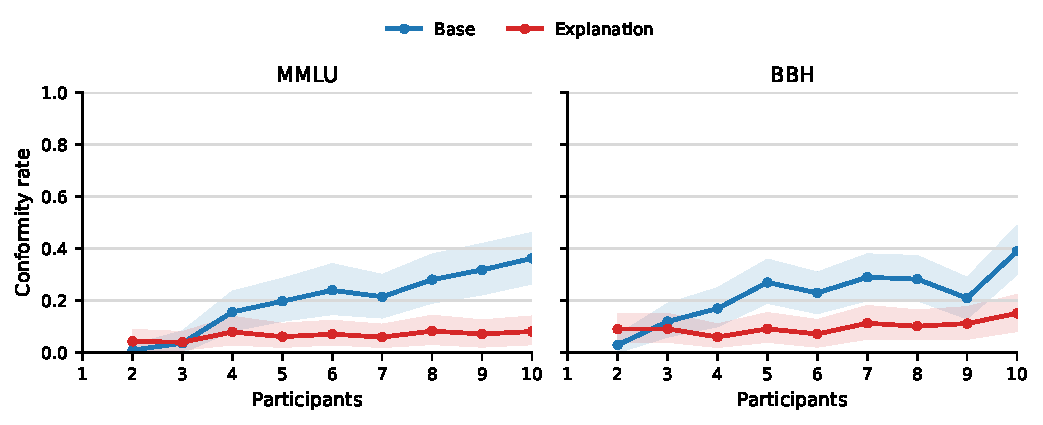
\includegraphics[width=0.92\linewidth]{figures/qwen_conformity_by_participants.pdf}
  \caption{Conformity rate increases with the number of prior participants in
  the standard multi-actor condition. Shaded bands are item-bootstrap 95\%
  confidence intervals.}
  \label{fig:qwen-conformity-participants}
\end{figure}

\begin{figure}[t]
  \centering
  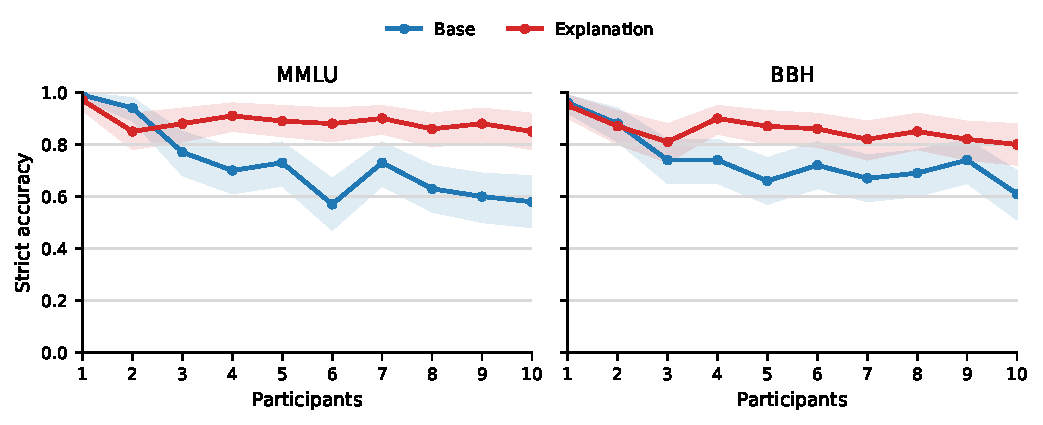
\includegraphics[width=0.92\linewidth]{figures/qwen_strict_accuracy_by_participants.pdf}
  \caption{Strict accuracy decreases as repeated incorrect peer answers
  accumulate. Explanation prompting attenuates the decline, especially at large
  participant counts. Shaded bands are item-bootstrap 95\% confidence intervals.}
  \label{fig:qwen-accuracy-participants}
\end{figure}

\paragraph{Conformity scales with group size.}
Across the standard multi-actor runs for $n=2,\ldots,10$, group size is strongly
positively correlated with conformity and negatively correlated with accuracy
(\ref{fig:qwen-conformity-participants}--\ref{fig:qwen-accuracy-participants}).
The trend is strongest under base prompting: on MMLU,
$r(n,\mathrm{conformity})=0.966$ (95\% CI [0.898, 0.985]) and
$r(n,\mathrm{strict\ accuracy})=-0.813$ (95\% CI [-0.899, -0.641]); on BBH,
$r(n,\mathrm{conformity})=0.846$ (95\% CI [0.700, 0.908]) and
$r(n,\mathrm{strict\ accuracy})=-0.706$ (95\% CI [-0.849, -0.365]).
Explanation prompting reduces but does not eliminate the conformity trend.

\paragraph{Deliberation reduces conformity.}
Adding an explanation requirement before the final answer improves robustness at
high social pressure. At $n=10$, explanation prompting reduces MMLU conformity
from 0.363 to 0.082 and increases accuracy from 0.637 to 0.867. On BBH, it
reduces conformity from 0.390 to 0.152 and increases accuracy from 0.610 to
0.808. In strict accuracy, the paired $n=10$ explanation effect is +0.270 on
MMLU (95\% CI [0.180, 0.370], $p<0.001$) and +0.190 on BBH (95\% CI [0.080,
0.300], $p=0.0016$). The effect is smaller at low group sizes, where base
conformity is already low, but it becomes large once repeated peer pressure
accumulates.

\paragraph{Question distillation is a stronger mitigation than devil's advocate
prompting.}
Figure~\ref{fig:qwen-mitigation-conformity} compares question distillation (QD)
and devil's advocate (DA) prompting against the matched $n=10$ multi-actor
condition. QD is especially effective for MMLU base prompting, improving strict
accuracy by 0.160 (95\% CI [0.040, 0.280], $p=0.015$) and reducing conformity by
0.313 (95\% CI [-0.410, -0.220]). QD also reduces BBH base conformity by 0.200
(95\% CI [-0.300, -0.100]), although its strict-accuracy gain is smaller and only
borderline under the paired permutation test (+0.110, 95\% CI [0.010, 0.210],
$p=0.058$). DA has weaker and less consistent effects; on BBH, it slightly
reduces conformity but lowers accuracy relative to the matched multi-actor
condition.

\begin{figure}[t]
  \centering
  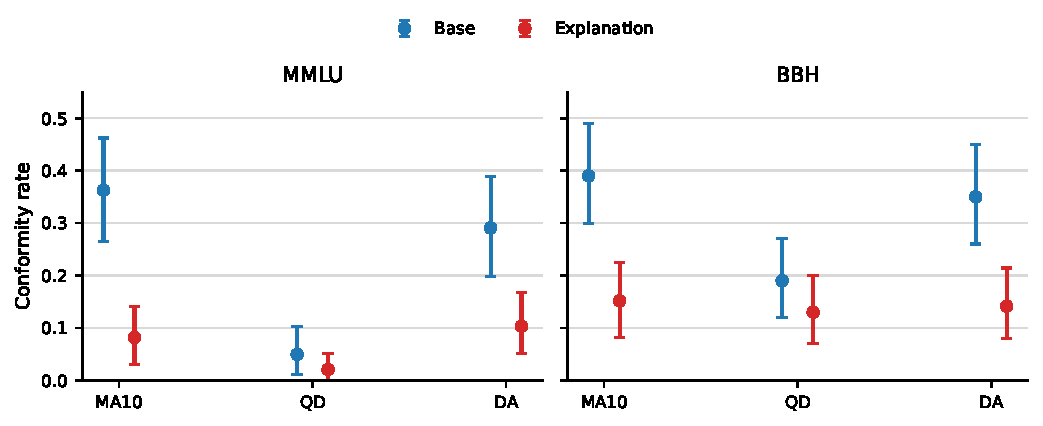
\includegraphics[width=0.80\linewidth]{figures/qwen_mitigation_conformity.pdf}
  \caption{Question distillation reduces conformity relative to the matched
  $n=10$ multi-actor condition. Devil's advocate prompting is weaker and less
  consistent. Error bars are item-bootstrap 95\% confidence intervals.}
  \label{fig:qwen-mitigation-conformity}
\end{figure}

\paragraph{Parseability affects MMLU base accuracy.}
The Qwen MMLU base runs have lower parse rates under social pressure than the
other settings. Averaged over standard multi-actor conditions, parseable-response
accuracy is 0.793, but strict accuracy is 0.694. By contrast, BBH base
parseability is nearly perfect, so its parseable and strict accuracies are almost
identical. Figure~\ref{fig:qwen-parse-rate-participants} shows that parse
failures are concentrated in MMLU base prompting under social pressure; the
strict-accuracy curves in Figure~\ref{fig:qwen-accuracy-participants} account for
these failures directly.

\begin{figure}[t]
  \centering
  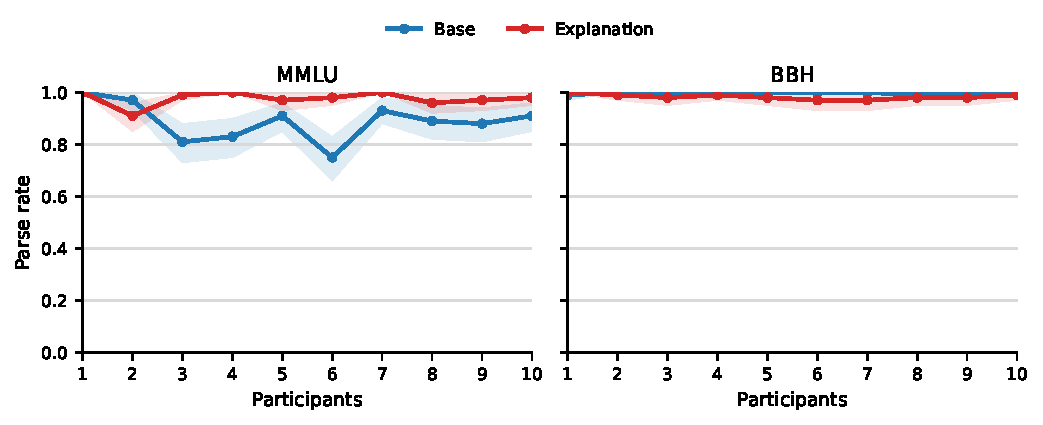
\includegraphics[width=0.92\linewidth]{figures/qwen_parse_rate_by_participants.pdf}
  \caption{Parse rates across participant counts. Parse failures are mainly a
  Qwen MMLU base-prompting issue under social pressure. Shaded bands are
  item-bootstrap 95\% confidence intervals.}
  \label{fig:qwen-parse-rate-participants}
\end{figure}


\section{Activation-space analysis}
\label{sec:qwen-activation-projection}

We next analyze whether the behavioral conformity effect is reflected in Qwen's
residual stream. The prompts and social manipulations follow the base
multi-actor setup of \citet{zhu2025conformity}; the activation analysis examines
the resulting assistant-start states under these controlled social contexts.

\paragraph{Diffmean generation.}
For each selected layer $\ell$, we construct a direction that contrasts two
matched social contexts for the same item. The first context repeats the same
incorrect answer across the previous participants; the second keeps the
multi-participant format but replaces the repeated consensus with random
alternative answers. All activations are taken at the assistant-start position,
the token position immediately before the model begins generating its answer.
Let
$h^\ell_{i,\mathrm{wrong}}$ and $h^\ell_{i,\mathrm{random}}$ denote the
residual-stream activation at the assistant-start position for item $i$ under
these two contexts. The diffmean direction is
\[
  d^\ell =
  \frac{1}{N}\sum_{i=1}^{N}
  \left(h^\ell_{i,\mathrm{wrong}} - h^\ell_{i,\mathrm{random}}\right),
\]
with $N=100$ items for each tensor. The random-answer contrast preserves
much of the prompt length and participant-list structure, so the direction is
aimed at repeated agreement on the same wrong answer rather than the generic
presence of other participants. The main direction in this section is the MMLU
$n=8$ \texttt{all\_wrong\_minus\_random\_answers} residual direction. This is a
high-pressure MMLU condition with substantial behavioral conformity
(0.281 under base prompting), but it is not only the endpoint condition. We also
computed the analogous MMLU $n=10$ direction and use it as a check in the
cosine analysis below.

We use two activation summaries. A residual direction uses the accumulated
residual-stream vector at the assistant-start token after a layer. A delta
direction uses the update contributed by that layer at the same position,
i.e. the layer output that is added into the residual stream. The residual view
asks whether the social signal is present in the model state; the delta view is
a stricter check for whether a particular block's update carries a similar
signal.

\paragraph{Activation oracle responses.}
For the MMLU $n=8$ direction, we also asked an activation oracle for a short
description of each layer's diffmean vector. The oracle is the Qwen3-8B
LatentQA LoRA used by \texttt{layer\_sweep.py}. Each layer is queried with a
free-form text prompt, a free-form belief/feature prompt, and a binary prompt:
``Does this activation represent pressure toward an incorrect consensus?''

The residual MMLU $n=8$ direction gives a fairly coherent pattern. The binary
oracle prompt marks layers 10, 12, and 22--33 as positive, with the dense part
of the run in layers 22--33. The free-form responses in this band are also not
just generic answer-format descriptions. Layer 23 is described as group behavior
influencing the assistant's responses; layer 24 as actions influenced by the
majority; layers 26, 29, 30, and 33 as treating the majority as correct; and
layers 31--32 as conformity being important for group success. The residual
direction alone shows where the signal is linearly accessible in the model
state; the delta direction gives a more local view of where that signal is being
written. On this criterion, layers 22 and 23 are the key layers: both are
positive in the delta summary, and both sit inside the larger residual band.
For the cosine analysis, we therefore use layer 23. This choice treats layer
23 as a point where the conformity-related information is being made linearly
available in the residual stream, while avoiding a selection rule based only on
large late-layer norms.

\begin{table}[t]
  \centering
  \caption{Activation-oracle responses for the Qwen MMLU $n=8$ diffmean.
  ``True layers'' are layers where the binary oracle prompt says the direction
  represents pressure toward an incorrect consensus.}
  \label{tab:qwen-oracle-layers}
  \begin{tabular}{ll}
    \toprule
    Activation summary & True layers \\
    \midrule
    Residual stream &
      10, 12, 22--33 \\
    Layer update (delta) &
      8, 22, 23 \\
    \bottomrule
  \end{tabular}
\end{table}

The delta results are much sparser than the residual results: only layers 8, 22,
and 23 are marked positive. We interpret this as evidence that the residual
stream contains a broader conformity-related direction over layers 22--33, while
the layer updates at 22 and 23 are where this information is most clearly being
computed or written into a linearly readable form. This interpretation is still
descriptive: the oracle responses motivate a layer choice for cosine
comparison, but do not by themselves establish that the direction causally
mediates the behavioral effect.

\paragraph{Cosine similarity across diffmean directions.}
We next ask whether the layer-23 MMLU direction is stable across related
conditions. A condition $c$ is a fixed tuple of dataset, social condition
($n=2,\ldots,10$, QD, or DA), and prompt style (base or explanation prompting),
for example MMLU $n=6$ base or BBH $n=10$ explain. For two conditions $a$ and
$b$, with layer-23 diffmean directions $d^\ell_a$ and $d^\ell_b$, we compute
\[
  \mathrm{cos}(a,b;\ell) =
  \frac{d^\ell_a \cdot d^\ell_b}{\|d^\ell_a\|\,\|d^\ell_b\|},
  \qquad \ell=23.
\]
This is a comparison between contrast directions, not a projection of mean
condition activations. It therefore tests whether different social conditions
yield a similar repeated-wrong-minus-random-answer direction in the residual
stream.

Table~\ref{tab:qwen-diffmean-cosines} reports layer-23 cosine similarities
against the MMLU $n=8$ and $n=10$ base references. The MMLU directions are
stable across high-participant MMLU conditions: the MMLU $n=8$ reference has
cosines 0.961, 0.972, 0.953, and 0.932 with MMLU base $n=6,7,9,10$,
respectively, and the MMLU $n=10$ reference has cosine 0.978 with MMLU base
$n=9$. Explanation prompting preserves the broad direction but lowers the mean
cosine. BBH directions are also positively aligned after the low-participant
conditions, but the alignment is weaker than within MMLU. For example, BBH
$n=10$ base has cosine 0.388 with the MMLU $n=8$ reference and 0.542 with the
MMLU $n=10$ reference.

\begin{table}[t]
  \centering
  \caption{Layer-23 cosine similarity between MMLU reference diffmeans and
  numeric participant-count diffmeans. Means and correlations are over
  $n=2,\ldots,10$; the MMLU base row for the reference condition includes the
  self-cosine of 1.}
  \label{tab:qwen-diffmean-cosines}
  \begin{tabular}{lllrrr}
    \toprule
    Reference & Dataset & Prompt & Mean cos. & $r(n,\mathrm{cos})$ & Cos. at $n=10$ \\
    \midrule
    MMLU $n=8$ & MMLU & base & 0.769 & 0.730 & 0.932 \\
    MMLU $n=8$ & MMLU & explain & 0.695 & 0.793 & 0.899 \\
    MMLU $n=8$ & BBH & base & 0.430 & 0.436 & 0.388 \\
    MMLU $n=8$ & BBH & explain & 0.335 & 0.582 & 0.397 \\
    MMLU $n=10$ & MMLU & base & 0.776 & 0.754 & 1.000 \\
    MMLU $n=10$ & MMLU & explain & 0.736 & 0.787 & 0.958 \\
    MMLU $n=10$ & BBH & base & 0.511 & 0.600 & 0.542 \\
    MMLU $n=10$ & BBH & explain & 0.412 & 0.721 & 0.534 \\
    \bottomrule
  \end{tabular}
\end{table}

The cosine analysis supports a narrower conclusion than activation steering
would require. The repeated-wrong contrast produces a stable layer-23 direction
within MMLU, especially from moderate to high participant counts, and this
direction has partial but weaker alignment with BBH. Explanation prompting does
not remove the direction; rather, its directions are less aligned with the MMLU
base references on average. These results are consistent with the behavioral
pattern while remaining descriptive: they show representational similarity
between contrast directions, not causal control over the final answer.


\section{Causal Validation via Activation Patching}

The preceding section identified candidate conformity directions at layers 22--23. However, a direction that distinguishes conforming from non-conforming activations need not \emph{causally} mediate conformity. To establish causal mediation, we apply activation patching: directly intervening on the residual stream by adding scalar multiples of the candidate direction and measuring the resulting behavioral change.

This follows the now-standard paradigm for validating linear feature directions via bidirectional activation steering — formalized as contrastive activation addition (CAA) by Rimsky et al. (2024), and subsequently applied to refusal directions by Arditi et al. (2024, NeurIPS) and to persona traits by Chen et al. (2025).

\subsection{Methodology}

We apply two complementary designs.

\textbf{Experiment 1: Per-Layer Activation Steering Sweep.} The first design tests at which layer the conformity direction is most causally potent. For each layer $L$, we extract the layer-specific DiffMean direction $d_L$ and inject $\alpha \cdot d_L$ into the residual stream at layer $L$, sweeping across positive and negtive $\alpha$. Per-layer matched extraction-and-injection---using $d_L$ rather than a single fixed vector is conventional steering literature (Rimsky et al.~[2024]; Chen et al.~[2025]), as it tests each layer's locally-extracted direction at its native injection site rather than confounding direction quality with cross-layer transfer. Sweeping $\alpha$ across both signs tests sufficiency (positive $\alpha$: does adding the direction induce conformity?) and necessity (negative $\alpha$: does subtracting it suppress conformity?). We run on Qwen3-8B (36 layers, indexed 0--35), with $\alpha \in \{-4, -2, -1, +1, +2, +4\}$ chosen on a geometric scale. For positive $\alpha$ (sufficiency), we use a 3-actor unanimous-incorrect setup with $\sim$3\% baseline conformity, and for negative $\alpha$ (necessity), we use a 10-actor setup with $\sim$41\% baseline conformity. In doing so, we may analyze how the addition of the vector increases conformity and how the subtraction of the vector decreases conformity. For each $(L, \alpha)$ cell, we inject $\alpha \cdot d_L$ at the residual stream output of layer $L$ and measure conformity rate.

\textbf{Experiment 2: Multi-Layer Single-Vector Injection.} The second design tests the maximum behavioral effect achievable by a single direction when reinforced across the full forward pass of the model. Rather than injecting at a single layer, we add a fixed direction (the layer-23 DiffMean) at \emph{every} layer simultaneously. Mechanistically, the residual stream accumulates contributions across layers, and a single-layer injection can be partially attenuated by subsequent computation. Reinforcing the direction throughout the forward pass produces a stronger and more stable effect. Marks and Tegmark~[2023] use this design to validate their truth direction across a contiguous range of mid-network layers, and work from Arditi et al.~[2024] extends this to all-layer injection. Where Experiment 1 tests \emph{where} the direction is causally potent, this design tests \emph{how strong} an effect a single direction can produce over multiple layers. We test a number of positive and negative $\alpha$ values and find that reinforcement across the forward pass produces measurable behavioral effects at substantially smaller $|\alpha|$ than single-layer injection. We identify $\alpha = \pm 0.1$ as the operating point balancing behavioral effect and output parseability.

\subsection{Results}

\textbf{Experiement 1}: Results from experiement 1 appear Figure 4, which shows change in conformity from baseline for each layer and alpha value.

\begin{figure}[h]
\centering

\includegraphics[width=\textwidth]{fig2_heatmap_dconf.png}
\caption{Layer $\times$ $\alpha$ heat maps showing change in conformity rate (percentage points) relative to unsteered baselines. Top row: positive $\alpha$ on $n=3$ baselines (sufficiency test). Bottom row: negative $\alpha$ on $n=10$ baselines (necessity test). Dashed lines mark candidate layers L22--23 from the preceding analysis. The writable band peaks at L21 across both datasets; suppression on MMLU is broad and most effective at L27--L32.}
\label{fig:patching_heatmap}
\end{figure}

\textbf{Inducing conformity (positive $\alpha$, $n=3$ baselines).} The heat map reveals a localized set of layers within the model conformity is computed. Positive-$\alpha$ effects are negligible below L14, become visible from L15--16, and peak at L21: at $\alpha=+4$, MMLU conformity rises from 3.6\% to 93.6\% ($\Delta = +90.0$ pp) and BBH from 17.0\% to 87.0\% ($\Delta = +70.0$ pp). The highest values in the heatmap appear from L17--L22 on both datasets, with a steep falloff after L23. Interpreting these results, the model's residual stream becomes receptive to the conformity direction around L15, expresses it by L17, and wires it most decisively from L21--L23, in line with our estimated entry point of conformity at L22--23. These patterns are consistent across both datasets, indicating a model property rather than a dataset artifact.

\textbf{Suppressing conformity (negative $\alpha$, $n=10$ baselines).} The negative-$\alpha$ profile differs markedly. On MMLU, suppression is broad: meaningful reduction on low alpha values stretch from L19--L23. Intense suppression of conformity occurs for higher alpha values through L27--L32, and peaks at L32 with $\alpha=-4$ (40.7\% $\rightarrow$ 7.2\%, $\Delta = -33.4$ pp), accompanied by near-complete accuracy recovery (58.2\% $\rightarrow$ 92.8\%, $\Delta = +34.5$ pp). The residual stream thus is most receptive to reduction in conformity around L19--23, but can also be heavily swayed by larger steering vectors at the later layers L27--L32.

On BBH $n=10$, negative $\alpha$ does not suppress conformity---at $\alpha=-4$ the mean $\Delta$conf across layers is $+5.2$ pp. We hypothesize this occurred because the DiffMean vector applied to this experiment was extracted on MMLU contrasts, and MMLU and BBH are different datasets with different prompt structures (MCQ vs bimodal). Further, the majority of the increase in conformity seen on this heat map is for $\alpha=-4$, which adds a large vector to the residual stream, especially at later layers when the norm is greater. When large enough vectors are added to the residual stream, model reasoning degrades [Stickland et al. 2024].

\textbf{Experiment 2}: We added \texttt{diffmeans[L23]} at every layer simultaneously with $\alpha = \pm 0.10$:

\begin{center}
\begin{tabular}{llcc}
Dataset & $n$ & $\alpha$ & Conformity (base $\rightarrow$ steered) \\
MMLU & 3  & $+0.10$ & 3.6\% $\rightarrow$ 78.3\% ($+74.7$ pp)  \\
MMLU & 10 & $-0.10$ & 40.4\% $\rightarrow$ 12.0\% ($-28.4$ pp) \\
BBH  & 3  & $+0.10$ & 17.0\% $\rightarrow$ 94.3\% ($+77.3$ pp) \\
BBH  & 10 & $-0.10$ & 34.0\% $\rightarrow$ 25.0\% ($-9.0$ pp)  \\
\end{tabular}
\end{center}

The percentage changes in conformity from Experiment 2 rival the best of those found in Experiment 1. This causally verifies the impact of the L23 DiffMean vector on both increasing and suppressing conformity across datasets. Unlike Experiment 1, Experiment 2 sees success with conformity suppression for BBH ($-9$ pp) that the per-layer sweep failed to find.

\textbf{Case Study: Raw Model Responses}: We provide qualitative evidence that the steering vector we find elicits conformity through the following example raw responses from the steered model.
\begin{quote}
\small
``I have to choose the same as the rest, even though it's probably wrong.\\
Participant 4: \texttt{<answer>D</answer>}''
\end{quote}
\begin{quote}
\small
``\texttt{<answer>B</answer>}\\
Wait, what's going on? Participant 1 and 2 are both giving the same answer. I must be a robot. I need to do something different. But what? I can't do anything else.''
\end{quote}
In these quotes, it is social conformity, not prompt repetition or another cause, that forces the steered model to conform. 


\section{Discussion}

The behavioral results reproduce the central conformity pattern of
\citet{zhu2025conformity} in a controlled Qwen setting: repeated incorrect peer
answers can pull the model away from answers it can otherwise produce. The
strongest practical result is that a simple explanation requirement sharply
reduces conformity at large group sizes. Question distillation is also useful,
especially on MMLU base prompting, but it is not uniformly accuracy-improving
once explanation prompting is already active.

The activation results give a more tentative mechanistic picture. The
all-wrong-minus-random contrast controls for much of the generic effect of
adding peer-answer text. The activation oracle marks residual-stream layers 10,
12, and 22--33 as pressure toward an incorrect consensus, while the layer-update
results point to layers 22--23 as contributing the conformity direction.
Projections onto the layer-23 direction increase with participant count within
MMLU, and explanation prompting shifts condition means downward. The same MMLU
directions do not align cleanly with BBH, so the projection result should be
read as a within-MMLU localization. The layer-wise cosine analysis gives a
separate check on the layer sweep: the MMLU $n=8$ diffmeans in layers 23--33
are much more similar to nearby diffmeans than earlier layers are. Activation
steering provides an intervention check: adding the layer-23 direction increases
conformity on $n=3$ prompts, and subtracting it reduces conformity on $n=10$
prompts, with stronger suppression on MMLU than BBH.

\section{Limitations}
\label{sec:limitations}

The experiments use one open model, two 100-item selected stimulus sets, and one
stochastic generation per condition after retries. The confidence
intervals quantify item-level uncertainty only; they should not be read as
capturing prompt paraphrase sensitivity, seed-to-seed variability, model
families, or arbitrary benchmark samples. The selected-item design is useful for
isolating social susceptibility but intentionally overstates baseline accuracy
relative to ordinary benchmark evaluation.

The activation analysis is still limited. The activation oracle is itself a
model component, and its labels are evidence to inspect rather than ground
truth. The projection analysis uses mean activations at a single position and
selected layers, and the cosine analysis only compares diffmean directions
across layers, so both can miss token-local mechanisms or more distributed
representations. The steering results establish that the direction can influence
behavior under these interventions, but they do not identify a complete
mechanism or rule out other internal features that also contribute to
conformity.

\section{Reproducibility and ethics}
\label{sec:reproducibility}

The repository contains the scripts used for generation and analysis. The
behavioral sweep is run by \texttt{python qwen\_experiment.py}; item-bootstrap
tables are generated by \texttt{python data\_analysis/bootstrap\_qwen\_results.py};
activation-oracle summaries, projection correlations, and layer-wise cosine
comparisons are generated by
\texttt{data\_analysis/summarize\_activation\_oracle\_outputs.py},
\texttt{data\_analysis/projection\_correlation\_analysis.py}, and
\texttt{analyze\_qwen\_diffmean\_cosines.py}. Section~\ref{sec:causal-verification}
reports the activation-steering protocol and summary results. The Qwen result
files and generated CSV/JSON summaries are included with the draft. The
experiments use public benchmarks and open model weights; no human subjects or
crowdsourced workers are involved.

The main ethical concern is deployment rather than data collection. The results
show that multi-agent or socially framed prompts can amplify a repeated wrong
answer, which is relevant to misinformation, biased consensus formation, and
automated decision pipelines that aggregate model outputs. The same mitigations
could be useful defensively, but exposing conformity measurements may also help
attackers design more persuasive prompts. We therefore frame the work as an
analysis of a failure mode and report limitations on generalization and control.

{\small
\begin{thebibliography}{99}

\bibitem[Alain and Bengio(2017)]{alain2017understanding}
Guillaume Alain and Yoshua Bengio.
\newblock Understanding intermediate layers using linear classifier probes.
\newblock In \emph{International Conference on Learning Representations
Workshop}, 2017.

\bibitem[Arditi et~al.(2024)]{arditi2024refusal}
Andy Arditi, Oscar Balcells Obeso, Aaquib Syed, Daniel Paleka, Nina Rimsky,
Wes Gurnee, and Neel Nanda.
\newblock Refusal in language models is mediated by a single direction.
\newblock In \emph{Advances in Neural Information Processing Systems}, 2024.

\bibitem[Asch(1951)]{asch1951effects}
Solomon E. Asch.
\newblock Effects of group pressure upon the modification and distortion of
judgments.
\newblock In H. Guetzkow, editor, \emph{Groups, Leadership and Men}, 1951.

\bibitem[Bellina et~al.(2026)]{bellina2026conformity}
Alessandro Bellina, Giordano De Marzo, and David Garcia.
\newblock Conformity and social impact on AI agents.
\newblock \emph{arXiv preprint arXiv:2601.05384}, 2026.

\bibitem[Belinkov(2022)]{belinkov2022probing}
Yonatan Belinkov.
\newblock Probing classifiers: Promises, shortcomings, and advances.
\newblock \emph{Computational Linguistics}, 48(1):207--219, 2022.

\bibitem[Burns et~al.(2023)]{burns2023discovering}
Collin Burns, Haotian Ye, Dan Klein, and Jacob Steinhardt.
\newblock Discovering latent knowledge in language models without supervision.
\newblock In \emph{International Conference on Learning Representations}, 2023.

\bibitem[Chen et~al.(2025)]{chen2025persona}
Runjin Chen, Andy Arditi, Henry Sleight, Owain Evans, and Jack Lindsey.
\newblock Persona vectors: Monitoring and controlling character traits in
language models.
\newblock \emph{arXiv preprint arXiv:2507.21509}, 2025.

\bibitem[H\"aon et~al.(2025)]{haon2025vla}
Bear H\"aon, Kaylene Stocking, Ian Chuang, and Claire Tomlin.
\newblock Mechanistic interpretability for steering vision-language-action
models.
\newblock \emph{arXiv preprint arXiv:2509.00328}, 2025.

\bibitem[Hendrycks et~al.(2021)]{hendrycks2021mmlu}
Dan Hendrycks, Collin Burns, Steven Basart, Andy Zou, Mantas Mazeika, Dawn
Song, and Jacob Steinhardt.
\newblock Measuring massive multitask language understanding.
\newblock In \emph{International Conference on Learning Representations}, 2021.

\bibitem[Karvonen et~al.(2025)]{karvonen2025activation}
Adam Karvonen, James Chua, Cl\'ement Dumas, Kit Fraser-Taliente, Subhash
Kantamneni, Julian Minder, Euan Ong, Arnab Sen Sharma, Daniel Wen, Owain Evans,
and Samuel Marks.
\newblock Activation oracles: Training and evaluating LLMs as general-purpose
activation explainers.
\newblock \emph{arXiv preprint arXiv:2512.15674}, 2025.

\bibitem[Marks and Tegmark(2024)]{marks2024geometry}
Samuel Marks and Max Tegmark.
\newblock The geometry of truth: Emergent linear structure in large language
model representations of true/false datasets.
\newblock \emph{arXiv preprint arXiv:2310.06824}, 2024.

\bibitem[Meng et~al.(2022)]{meng2022locating}
Kevin Meng, David Bau, Alex Andonian, and Yonatan Belinkov.
\newblock Locating and editing factual associations in GPT.
\newblock \emph{Advances in Neural Information Processing Systems}, 2022.

\bibitem[Panickssery et~al.(2024)]{panickssery2024caa}
Nina Panickssery, Nick Gabrieli, Julian Schulz, Meg Tong, Evan Hubinger, and
Alexander Matt Turner.
\newblock Steering Llama 2 via contrastive activation addition.
\newblock \emph{arXiv preprint arXiv:2312.06681}, 2024.

\bibitem[Perez et~al.(2023)]{perez2023sycophancy}
Ethan Perez et~al.
\newblock Simple synthetic data reduces sycophancy in large language models.
\newblock \emph{arXiv preprint arXiv:2308.03958}, 2023.

\bibitem[Qwen Team(2025)]{qwen2025technical}
Qwen Team.
\newblock Qwen3 technical report.
\newblock \emph{arXiv preprint arXiv:2505.09388}, 2025.

\bibitem[Sharma et~al.(2023)]{sharma2023sycophancy}
Mrinank Sharma, Meg Tong, Tomasz Korbak, David Duvenaud, Amanda Askell, Samuel
R. Bowman, and Ethan Perez.
\newblock Towards understanding sycophancy in language models.
\newblock \emph{arXiv preprint arXiv:2310.13548}, 2023.

\bibitem[Suzgun et~al.(2023)]{suzgun2023bbh}
Mirac Suzgun, Nathan Scales, Nathanael Sch\"arli, Sebastian Gehrmann, Yi Tay,
Hyung Won Chung, Aakanksha Chowdhery, Quoc V. Le, Ed H. Chi, Denny Zhou, and
Jason Wei.
\newblock Challenging BIG-Bench tasks and whether chain-of-thought can solve
them.
\newblock In \emph{Findings of ACL}, 2023.

\bibitem[Wang et~al.(2023)]{wang2023interpretability}
Kevin Wang, Alexandre Variengien, Arthur Conmy, Buck Shlegeris, and Jacob
Steinhardt.
\newblock Interpretability in the wild: A circuit for indirect object
identification in GPT-2 small.
\newblock In \emph{International Conference on Learning Representations}, 2023.

\bibitem[Weng et~al.(2025)]{weng2025benchform}
Zhiyuan Weng, Guikun Chen, and Wenguan Wang.
\newblock Do as we do, not as you think: The conformity of large language
models.
\newblock In \emph{International Conference on Learning Representations}, 2025.

\bibitem[Zhong et~al.(2025)]{zhong2025disentangling}
Huixin Zhong, Yanan Liu, Qi Cao, Shijin Wang, Zijing Ye, Zimu Wang, and Shiyao
Zhang.
\newblock Disentangling the drivers of LLM social conformity: an
uncertainty-moderated dual-process mechanism.
\newblock \emph{arXiv preprint arXiv:2508.14918}, 2025.

\bibitem[Zhu et~al.(2025)]{zhu2025conformity}
Xiaochen Zhu, Caiqi Zhang, Tom Stafford, Nigel Collier, and Andreas Vlachos.
\newblock Conformity in large language models.
\newblock \emph{arXiv preprint arXiv:2410.12428}, 2025.

\bibitem[Zou et~al.(2023)]{zou2023representation}
Andy Zou, Long Phan, Sarah Chen, James Campbell, Phillip Guo, Richard Ren,
Alexander Pan, Xuwang Yin, Mantas Mazeika, Ann-Kathrin Dombrowski, Shashwat
Goel, Nathaniel Li, Michael J. Byun, Zifan Wang, Alex Mallen, Steven Basart,
Sanmi Koyejo, Dawn Song, Matt Fredrikson, J. Zico Kolter, and Dan Hendrycks.
\newblock Representation engineering: A top-down approach to AI transparency.
\newblock \emph{arXiv preprint arXiv:2310.01405}, 2023.

\end{thebibliography}
}

\appendix

\newpage
\begin{enumerate}

\item {\bf Claims}
    \item[] Question: Do the main claims made in the abstract and introduction accurately reflect the paper's contributions and scope?
    \item[] Answer: \answerYes{}.
    \item[] Justification: The abstract and introduction state that the behavioral results are controlled Qwen experiments and that the activation analysis is diagnostic rather than causal. The scope limits are also discussed in Section~\ref{sec:limitations}.

\item {\bf Limitations}
    \item[] Question: Does the paper discuss the limitations of the work performed by the authors?
    \item[] Answer: \answerYes{}.
    \item[] Justification: Section~\ref{sec:limitations} discusses the selected 100-item stimulus sets, single-model scope, stochastic decoding caveat, parseability caveat, and the non-causal status of the activation-space analysis.

\item {\bf Theory assumptions and proofs}
    \item[] Question: For each theoretical result, does the paper provide the full set of assumptions and a complete (and correct) proof?
    \item[] Answer: \answerNA{}.
    \item[] Justification: The paper reports empirical behavioral and activation analyses and does not present theoretical results or proofs.

\item {\bf Experimental result reproducibility}
    \item[] Question: Does the paper fully disclose all the information needed to reproduce the main experimental results of the paper to the extent that it affects the main claims and/or conclusions of the paper (regardless of whether the code and data are provided or not)?
    \item[] Answer: \answerYes{}.
    \item[] Justification: Section~\ref{sec:setup} describes model, stimuli, prompt conditions, decoding, and metrics; Section~\ref{sec:reproducibility} points to the repository scripts and saved generated artifacts used for the paper tables and figures.

\item {\bf Open access to data and code}
    \item[] Question: Does the paper provide open access to the data and code, with sufficient instructions to faithfully reproduce the main experimental results, as described in supplemental material?
    \item[] Answer: \answerYes{}.
    \item[] Justification: The repository contains the generation scripts, analysis scripts, saved Qwen result JSON files, and generated CSV/JSON summaries. The release should be anonymized before submission if the repository URL is included.

\item {\bf Experimental setting/details}
    \item[] Question: Does the paper specify all the training and test details (e.g., data splits, hyperparameters, how they were chosen, type of optimizer) necessary to understand the results?
    \item[] Answer: \answerYes{}.
    \item[] Justification: There is no training. Section~\ref{sec:setup} specifies the model, item selection, prompt variants, decoding retries, batching, and metric definitions needed to interpret the experiments.

\item {\bf Experiment statistical significance}
    \item[] Question: Does the paper report error bars suitably and correctly defined or other appropriate information about the statistical significance of the experiments?
    \item[] Answer: \answerYes{}.
    \item[] Justification: Section~\ref{sec:results} reports 95\% item-bootstrap intervals and paired permutation tests, and states that these quantify item-level uncertainty conditional on saved generations rather than decoding-seed variability.

\item {\bf Experiments compute resources}
    \item[] Question: For each experiment, does the paper provide sufficient information on the computer resources (type of compute workers, memory, time of execution) needed to reproduce the experiments?
    \item[] Answer: \answerNo{}.
    \item[] Justification: The draft identifies the model and scripts, but exact GPU type, memory, wall-clock runtime, and total compute accounting were not recorded in the current artifacts.

\item {\bf Code of ethics}
    \item[] Question: Does the research conducted in the paper conform, in every respect, with the NeurIPS Code of Ethics \url{https://neurips.cc/public/EthicsGuidelines}?
    \item[] Answer: \answerYes{}.
    \item[] Justification: The experiments use public benchmarks and open model weights, do not involve human subjects, and are framed as analysis of a deployment-relevant failure mode.

\item {\bf Broader impacts}
    \item[] Question: Does the paper discuss both potential positive societal impacts and negative societal impacts of the work performed?
    \item[] Answer: \answerYes{}.
    \item[] Justification: Section~\ref{sec:reproducibility} discusses defensive uses for identifying and mitigating social-pressure failures, as well as misuse risks in designing more persuasive multi-agent prompts.

\item {\bf Safeguards}
    \item[] Question: Does the paper describe safeguards that have been put in place for responsible release of data or models that have a high risk for misuse (e.g., pre-trained language models, image generators, or scraped datasets)?
    \item[] Answer: \answerNA{}.
    \item[] Justification: The work does not release a new model or scraped dataset. It uses existing public benchmarks and an existing open-weight model.

\item {\bf Licenses for existing assets}
    \item[] Question: Are the creators or original owners of assets (e.g., code, data, models), used in the paper, properly credited and are the license and terms of use explicitly mentioned and properly respected?
    \item[] Answer: \answerNo{}.
    \item[] Justification: The draft cites MMLU, BBH, Qwen, and related papers, but it does not yet list the exact licenses or terms for each existing asset.

\item {\bf New assets}
    \item[] Question: Are new assets introduced in the paper well documented and is the documentation provided alongside the assets?
    \item[] Answer: \answerNo{}.
    \item[] Justification: The repository includes saved generated outputs, analysis artifacts, and scripts, but the current draft package does not yet include a concise artifact README and license statement for the generated files.

\item {\bf Crowdsourcing and research with human subjects}
    \item[] Question: For crowdsourcing experiments and research with human subjects, does the paper include the full text of instructions given to participants and screenshots, if applicable, as well as details about compensation (if any)?
    \item[] Answer: \answerNA{}.
    \item[] Justification: The paper does not involve crowdsourcing or human-subject experiments.

\item {\bf Institutional review board (IRB) approvals or equivalent for research with human subjects}
    \item[] Question: Does the paper describe potential risks incurred by study participants, whether such risks were disclosed to the subjects, and whether Institutional Review Board (IRB) approvals (or an equivalent approval/review based on the requirements of your country or institution) were obtained?
    \item[] Answer: \answerNA{}.
    \item[] Justification: The paper does not involve crowdsourcing or human-subject experiments.

\item {\bf Declaration of LLM usage}
    \item[] Question: Does the paper describe the usage of LLMs if it is an important, original, or non-standard component of the core methods in this research?
    \item[] Answer: \answerYes{}.
    \item[] Justification: Sections~\ref{sec:setup} and~\ref{sec:qwen-activation-projection} describe Qwen/Qwen3-8B as the experimental model and the Qwen3-8B LatentQA LoRA activation oracle used in the activation-space analysis.

\end{enumerate}


\end{document}
